\documentclass[12pt,a4paper]{article}
\usepackage[utf8]{inputenc}
\usepackage[T1]{fontenc}
\usepackage{amsmath}
\usepackage{amssymb}
\usepackage{float}
\usepackage{graphicx}
\title{CAD-Schulung}
\author{Mirco Huber}
\date{31.01.2023}
\begin{document}
	\maketitle
	\newpage
	\section{Konfigurationen}
	Solidworks bietet die Möglichkeit, innerhalb einer Datei, beispielsweise eines Parts, einzelne Parameter zu variieren. Im Folgenden wird dieses Feature anhand einer Schraube genauer angeschaut.
	\subsection{Anwendungsmöglichkeit / Zweck}
	Gerade bei Normteilen wie Schrauben oder Muttern ist es von Vorteil, nicht immer wieder den Schraubenkopf o.Ä. modellieren zu müssen, nur um eine neue Schraubenlänge abzubilden. Dies kann zwar auch durch Kopieren und anschliessendem Anpassen einer \lq Masterdatei\rq erreicht werden, jedoch sind dann diese Dateien nicht mehr verknüpft, sollte man doch mal bei einer ganzen Schraubenfamilie eine Eigenschaft anpassen müssen (z.B. Färbung, um Oberflächenbeschaffenheit zu visualisieren). Hier kommen Konfigurationen zum Tragen: Eine Schraubenart wie beispielsweise die Philips H Senkkopfschrauben BN388 muss nur einmal modelliert werden; die unterschiedlichen Gewindelängen können anschliessend über Konfigurationen erzeugt werden. 
	\subsection{Anlegen von Konfigurationen}
	In der Abbildung \ref{fig:Skizze} ist eine mögliche Art visualisiert, wie die Senkschraube mit einer rotierenden Skizze modelliert werden kann. Innerhalb der Schraubenfamilie MN388 sind alle Dimensionen bis auf die Gewindelänge bei gegebenem Gewindedurchmesser konstant. Daher wird im Folgenden primär darauf eingegangen, wie die Gewindelänge parametriert und somit Konfigurationen für unterschiedliche Gewindelängen angelegt werden kann.
	\begin{figure}[H]
		\centering
		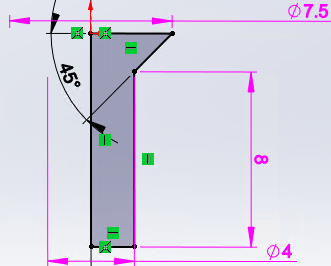
\includegraphics[width=.4\linewidth]{310123_CAD_PDM/screenshot003}
		\caption{Skizze zum Anlegen von Konfigurationen}
		\label{fig:Skizze}
	\end{figure}
	\noindent
	Durch Doppelklick auf das Mass für die Gewindelänge (hier 8mm) öffnet sich eine Maske, um dieses zu modifizieren. An dieser Stelle ist zu Empfehlen, dem Mass einen klingenden Namen zu geben. Im folgenden ist dieses Mass auf \textit{L\_Gewinde} (siehe \ref{fig:screenshot004}) benannt. Das \textit{L} ist hierbei ein Indikator, dass es sich um eine Länge handelt. Als Konvention empfielt es sich, gängige Präfixe wie \textit{D} für Aussendurchmesser, \textit{d} für Innendurchmesser oder \textit{t} für Dicke (engl. thickness) zu verwenden. Dies hilt, zu einem späteren Zeitpunkt zu erkennen, welches Mass konfiguriert werden soll, da in der dafür benötigten Ansicht / Tabelle nur die Namen der Masse zu sehen sind
	\begin{figure}[H]
		\centering
		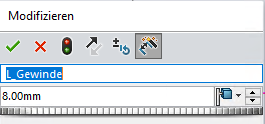
\includegraphics[width=.4\linewidth]{310123_CAD_PDM/screenshot004}
		\caption{}
		\label{fig:screenshot004}
	\end{figure}\noindent
	Ist die Zeichnug fertig / vollständig bemasst, kann der Volumenkörper aus Rotationsaufsatz erzeugt werden. Weiter kann das Schraubenkopfprofil modelliert werden. Anschliessend steht die Konfiguration weiterer Schraubenlängen an. Hierfür muss das Feature, welchem die zu konfigurierende Skizze zugrunde liegt, mit der rechten Maustaste angewählt werden. Es öffnet sich ein Kontextmenu, welches die Option \textit{Feature konfigurieren} anbietet:
	\begin{figure}[H]
		\centering
		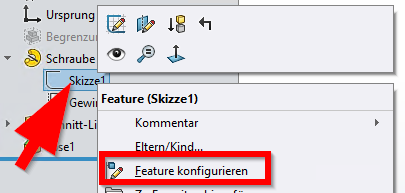
\includegraphics[width=.6\linewidth]{310123_CAD_PDM/screenshot005}
		\caption{}
		\label{fig:screenshot005}
	\end{figure}\noindent
	\noindent
	Es öffnet sich ein Dialog, welcher pro Mass dieser Skizze eine Spalte erstellt. Der Spaltenname korrespondiert hierbei mit dem Namen, der dem Mass zuvor in der Skizze vergeben wurde (!).
	\begin{figure}[H]
		\centering
		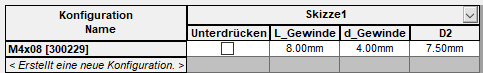
\includegraphics[width=.6\linewidth]{310123_CAD_PDM/screenshot006}
		\caption{}
		\label{fig:Konfigtabelle}
	\end{figure}\noindent
	Durch Klicken in das graue Feld < Erstellt eine neue Konfiguration > können beliebige weitere Konfigurationen angelegt werden. 
	\subsection{Verwenden von Konfigurationen}
	Ein weiterer Vorteil nebst der Tatsache, dass die Schraubengeometrie nur einmal modelliert aber dennoch für alle Konfigurationen in einem Atemzug angepasst werden kann, liegt in der Verwendung dieses Parts in Baugruppen: wird ein Part, welches über Konfigurationen verfügt, in eine Baugruppe eingefügt, öffnet sich sofort ein Dialogfenster, welches alle vorhandenen Konfigurationen anzeigt. Diese werden jeweils in alfabetischer Reihenfolge angezeigt, weshalb es durchaus Sinn macht, die Konfigurationsnamen mit Hinblick auf diese Anwendung zu wählen. Bei den Schrauben bietet es sich hier beispielsweise an, diese nach dem Schema \textit{Nenndurchmesser}x\textit{Gewindelänge} zu benennen, wobei es hier weiter Sinn macht, einstellige Gewindelängen um eine führende \texttt{0} zu ergänzen. Anderenfalls kommt die Länge 10 vor der Länge 3. 
	\begin{figure}[H]
		\centering
		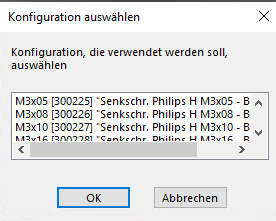
\includegraphics[width=.4\linewidth]{310123_CAD_PDM/screenshot007}
		\caption{Konfigurationsauswahl beim Einfügen in eine Baugruppe}
		\label{fig:screenshot007}
	\end{figure}
	 
	
	
	\section{Solidworsdateien: Metadaten}
	Solidworks verfügt über ein eigenes, proprietäres Sortiment an Dateiformaten für die verschiedenen Dateitypen wie Zeichnungen (.dwg), Einzelteile (.prt) oder Baugruppen (.asm). Diese Dateitypen ermöglichen, die eigentlichen Daten mit \textit{Metadaten} anzureichern. Auf jeder der Solidworks-Datein können beliebige Attribute im Rahmen eines \textit{Key-Value-Paares} abgelegt werden. Diese Metadaten können in Zeichnungen, Stücklisten oder PDM-Suchfiltern verwendet werden. 
	Die Metadaten können über eine Schaltfläche in der Kopfleiste von Solidworks (siehe Screenshot \ref{fig:metadataDialog})  geöffnet werden.
	\subsection{Anlegen und ändern von Metadaten}
	\begin{figure}[H]
		\centering
		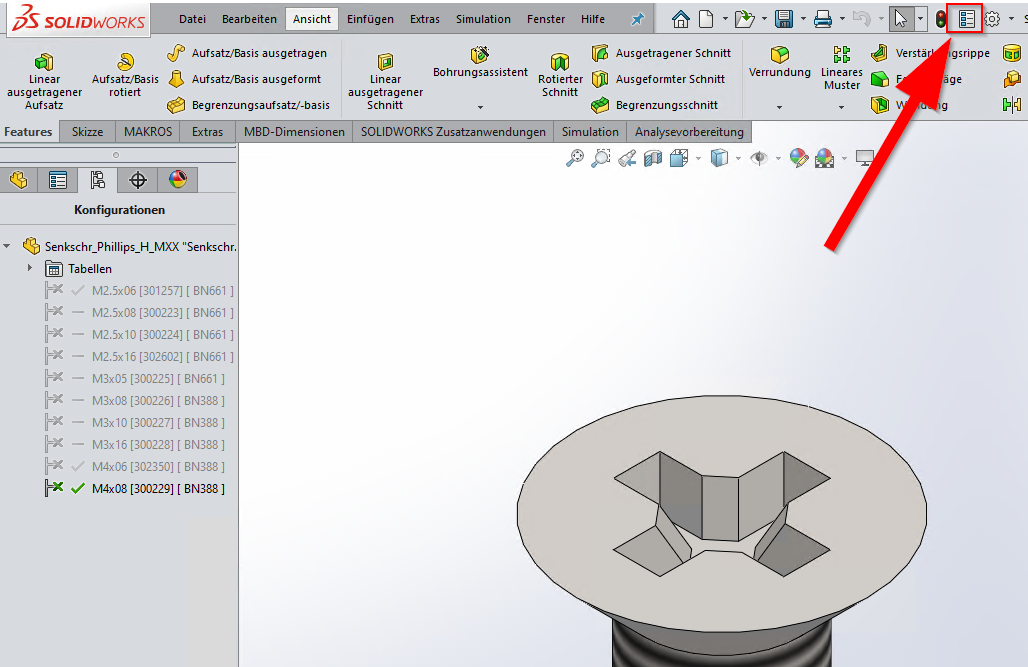
\includegraphics[width=1\linewidth]{310123_CAD_PDM/screenshot001}
		\caption[Solidworks-Metadaten abfragen / editieren]{Solidworks-Metadaten abfragen / editieren}
		\label{fig:metadataDialog}
	\end{figure}
	Im geöffneten Dialog werden die aktuell vorhandenen Metadaten angezeigt. Hierbei ist zu beachten, dass Solidworks zwischen Metadaten auf der gesamten Datei (Tab \textit{Benutzerdefiniert}) sowie solchen, die konfigurationsgebunden sind (Tab \textit{Konfigurationsspezifisch}) unterscheidet. Bei letzteren ist darauf zu achten, dass im Dropdownmenu \textit{Anwenden auf} die richtige Konfiguration gewählt ist. Die Tabs sind in der Abbildung \ref{fig:screenshot002} hervorgehoben.
	\begin{figure}
		\centering
		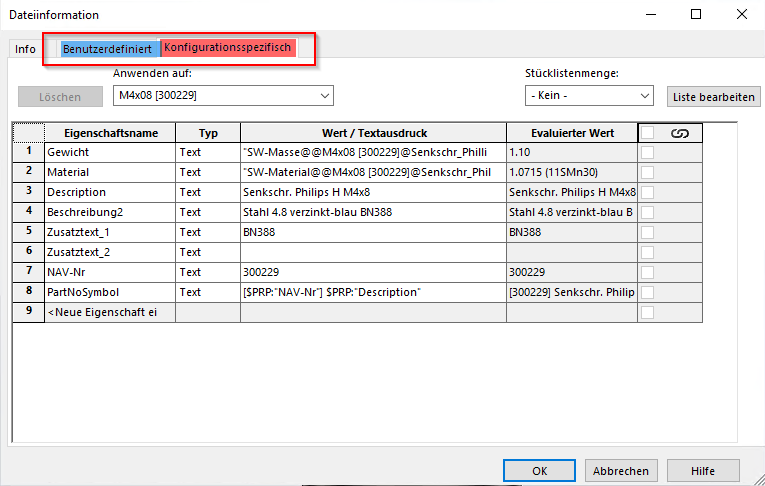
\includegraphics[width=1\linewidth]{310123_CAD_PDM/screenshot002}
		\caption{}
		\label{fig:screenshot002}
	\end{figure}
	\subsection{Metadaten: Textausdruck vs. Evaluierter Wert}
	Die Metadaten werden als Key-Value-Paare abgelegt. Als Key (\textit{Eigenschaftsname}) kann ein beliebiger Text eingegeben werden, welchem dann der Wert aus der Spalte Wert/Textausdruck (Value) zugewiesen wird. Die gesamten Metadaten dienen anschliessend als Lookup-Table: Wird ein Key geeignet referenziert, kann Solidworks den zu diesem Key gehörenden Value in dieser Lookup-Table abrufen. Wichtig hierbei ist, dass der Key-Text \textbf{sinnvoll, sprechend, eindeutig und fehlerfrei} ist. Als Value kann ein expliziter Wert oder eine Verknüpfung von vorhandenen Werten eingetragen werden. Um einen Wert zu referenzieren, muss dieser wie folgt referenziert werden:
	\begin{equation*}
		\$PRP:"Key-Bezeichnung"
	\end{equation*} 
	\textbf{Beachte: } die doppelten Anführungszeichen müssen geschrieben werden. Solidworks erkennt anhand der Zeichenfolge \textit{\$PRP}, dass ein vorhandener Key abgefragt werden soll. Der \textbf{genaue} Key / Name des Parameters wird zwischen doppelten Anführungszeichen gesucht.\\
	Sind beispielsweise die beiden die Keys \textit{NAV-Nr} und \textit{Description} bereits vorhanden, kann beispielsweise folgender Ausdruck einem neuen Key zugewiesen werden:
	\begin{eqnarray*}
		[\$PRP:"NAV-Nr"] \$PRP:"Description"
	\end{eqnarray*}
	\begin{table}[H]
		\centering
		\caption{Beispiele für Key-Value-Paare}
		\begin{tabular}{|c|c|}
			\hline
			Key (Eigenschaftsname) & Value (Wert/Textausdruck) \\
			\hline
			NAV-Nr & 300229 \\
			\hline
			Description & Senkschr. Philips H M4x8 \\
			\hline
		\end{tabular}
	\end{table}
\noindent
	Wenn die Metadaten wie in Tabelle aussehen, resultiert aus dem obigen Textausdruck 
	\begin{equation*}
		\text{[300229] Senkschr. Philips H M4x8}
	\end{equation*}
	Diese Formel kann beispielsweise auf der Vorlage für Parts definiert werden. Sobald ein neues Bauteil mit dieser Vorlage angelegt wird, ist diese Formel bereits vorhanden. Durch abfüllen der Keys \textit{NAV-Nr} und \textit{Description} erhält man diesen formatierten Text automatisch und kann diesen beispielsweise in Zeichnungen wieder abfragen.
	\section{Drawings: \$PRP vs. \$PRPSHEET}
	Auch Zeichnungen (.dwg) bieten die Möglichkeit, diese Dateien mit Metadaten anzureichern. Jedoch macht es häufig Sinn, auf die Metadaten der in den Zeichnungen referenzierten Volumenmodelle zurückzugreifen. Hierfür unterscheidet Solidworks die Lookup-Tabellen mittels Präfix \textit{\$PRP} bzw. \textit{\$PRPSHEET}: Während Solidworks Values zu Keys mit dem Präfix \$PRPin den Metadaten der jeweiligen Zeichnung sucht, greift es bei Values mit dem Präfix \$PRPSHEET auf die Lookup-Table des Volumenmodells, welches als "Hauptansicht" in den Eigenschaften der Zeichnung angegeben wurde, zurück. Die Haupansicht kann festgelegt werden, indem in der Zeichnung mittels rechter Maustaste ins Leere geklickt und anschliessend \textit{Eigenschaften...} angeklickt wird.
	\begin{figure}[H]
		\centering
		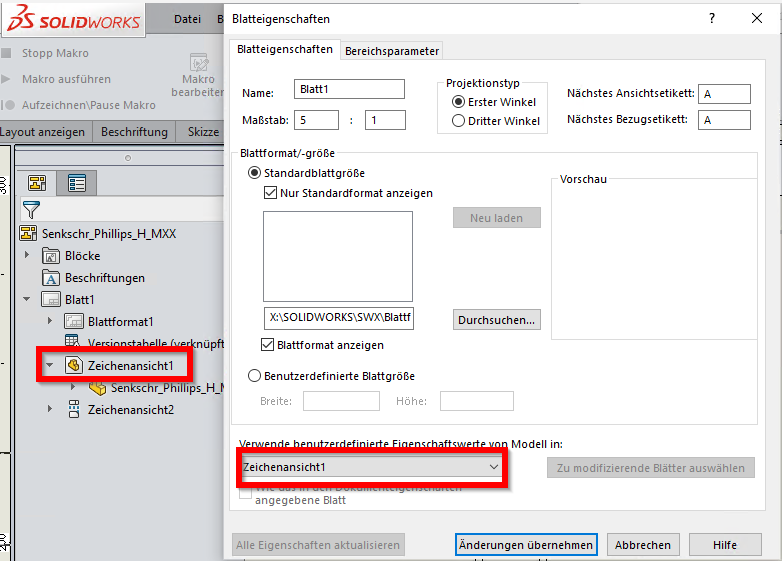
\includegraphics[width=.5\linewidth]{310123_CAD_PDM/screenshot008}
		\caption{Einstellung der "Hauptansicht"}
		\label{fig:screenshot008}
	\end{figure}\noindent
	Somit kann im Zeichnungskopf an jeweils sinnvollen Stellen mit diesen Platzhaltern gearbeitet werden. Ist dies (einigermassen) sinnvoll umgesetzt, erscheint der Kopf zu erst leer, da noch keine "Hauptansicht" definiert ist. Wird eine Zeichnungansicht durch Einfügen einer Projektion eines Volumenkörpers angelegt, ist dies automatisch die Hauptansicht. Der Kopf wird daher automatisch mit den Values zu den Keys aus dem Kopf ausgefüllt, indem die Metadaten des Volumenkörpers danach abgefragt werden. Dieser Effekt kann in der Abbildung \ref{fig:screenshot009} gesehen werden.
	\begin{figure}[H]
		\centering
		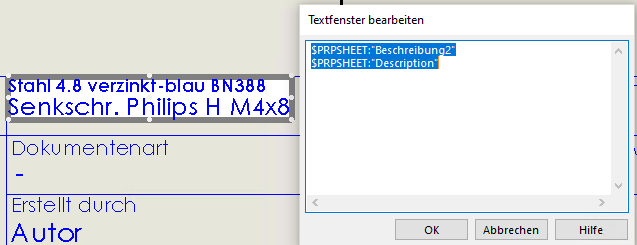
\includegraphics[width=1\linewidth]{310123_CAD_PDM/screenshot009}
		\caption{Vergleich Platzhalter / Zeichnungskopf}
		\label{fig:screenshot009}
	\end{figure}
	
\end{document}